%%%%%%%%%%%%%%%%%%%%%%%%%%%%%%%%%%%%%%%%%%%%%%%%%%%%%%%%%%%%%%%%%%%%%%%%%%%%%%%%
\documentclass[twocolumn]{revtex4}

%%%%%%%%%%%%%%%%%%%%%%%%%%%%%%%%%%%%%%%%%%%%%%%%%%%%%%%%%%%%%%%%%%%%%%%%%%%%%%%%
% Note that comments begin with a "%" and are not turned into text in the .pdf
% document.
%%%%%%%%%%%%%%%%%%%%%%%%%%%%%%%%%%%%%%%%%%%%%%%%%%%%%%%%%%%%%%%%%%%%%%%%%%%%%%%%

%%%%%%%%%%%%%%%%%%%%%%%%%%%%%%%%%%%%%%%%%%%%%%%%%%%%%%%%%%%%%%%%%%%%%%%%%%%%%%%%
% Include some extra packages.
%%%%%%%%%%%%%%%%%%%%%%%%%%%%%%%%%%%%%%%%%%%%%%%%%%%%%%%%%%%%%%%%%%%%%%%%%%%%%%%%
\usepackage[]{graphicx}
%%%%%%%%%%%%%%%%%%%%%%%%%%%%%%%%%%%%%%%%%%%%%%%%%%%%%%%%%%%%%%%%%%%%%%%%%%%%%%%%

%%%%%%%%%%%%%%%%%%%%%%%%%%%%%%%%%%%%%%%%%%%%%%%%%%%%%%%%%%%%%%%%%%%%%%%%%%%%%%%%
\begin{document}

%%%%%%%%%%%%%%%%%%%%%%%%%%%%%%%%%%%%%%%%%%%%%%%%%%%%%%%%%%%%%%%%%%%%%%%%%%%%%%%%
\title{
Journal article
}

\author{Sachin Vohra}
\affiliation{Siena College, Loudonville, NY}

\date{\today}

\begin{abstract}
\section{Abstract}
The motivation for this project was that it is counted as out Final Exam. If I do well on this 
    project, I will have a better final grade in the class.The goal of this assignment was to figure out 
    when a Velociraptor going at 18 m/s would catch up to a Human going at 3 m/s with a 30 meter head 
    start. Then we had to calculate at what time is the Velociraptor one meter behind the Human. Lastly,
    we had to find out the probability of the Human surviving, using the given information. The point of 
    this analysis is to show that we understand the Final Project. 
    
\end{abstract}

\maketitle
%%%%%%%%%%%%%%%%%%%%%%%%%%%%%%%%%%%%%%%%%%%%%%%%%%%%%%%%%%%%%%%%%%%%%%%%%%%%%%%%

%%%%%%%%%%%%%%%%%%%%%%%%%%%%%%%%%%%%%%%%%%%%%%%%%%%%%%%%%%%%%%%%%%%%%%%%%%%%%%%%
\section{Plots}
%%%%%%%%%%%%%%%%%%%%%%%%%%%%%%%%%%%%%%%%%%%%%%%%%%%%%%%%%%%%%%%%%%%%%%%%%%%%%%%%
\begin{figure}[h]
	\centering 
	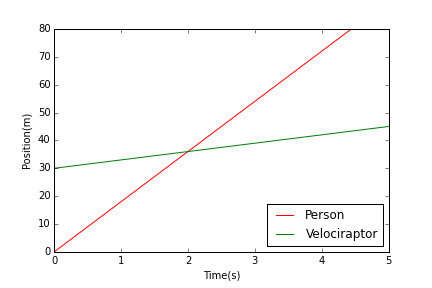
\includegraphics[width=0.5\textwidth] {PositionVsTime.png}
	\caption{This is the graph for number one.\label{figure:Graph}}
\end{figure}
First, I used for loops with the given information to eventually produce a graph.
Then, I used a previous lab to guide me through the process of producing a graph. By examining the 
graph, I realized that the Velociraptor and the human meet at about two seconds. 

%%%%%%%%%%%%%%%%%%%%%%%%%%%%%%%%%%%%%%%%%%%%%%%%%%%%%%%%%%%%%%%%%%%%%%%%%%%%%%%%
\section{Number Two}
%%%%%%%%%%%%%%%%%%%%%%%%%%%%%%%%%%%%%%%%%%%%%%%%%%%%%%%%%%%%%%%%%%%%%%%%%%%%%%%%
First, I stated "for x in time:" Then I typed two equations: p = 3 * x + 30 and v = 18 * x and then set p equal to v. Lastly, I used a print statement to determine that they meet at 2.0 seconds.
	\subsection{Algebra}
Given 
$$X_R_i = 0 (m)$$		
$$V_R_i = 18 (m/s)$$	
$$X_H_i = 30(m)$$
$$V_H_i = 3 (m/s)$$
$$a = 0 (m/s^2)$$

$$X_R_f = X_R_i + V_R_i(t) + .5(a)(t^2)$$	
$$X_R_f = V_R_i(t)$$						
$$X_H_f = X_H_i + V_H_i(t) + .5(a)(t^2)$$
$$X_H_f = X_H_i + V_H_i(t)$$
$$X_R_f = X_H_f$$ 
$$V_R_i(t) = X_H_i + V_H_i(t)$$
$$V_R_i(t) - V_H_i(t) = X_H_i$$
$$t(V_R_i - V_H_i) = X_H_i$$
$$t = X_H_i / (V_R_i - V_H_i)$$
$$t = 30 / (18 - 3)$$
$$t = 2(s)$$ 

\section{Number Three}
 I used the same approach as number two to calculate the time when the Velociraptor is one meter behind the Human. The time I received was 2.0 seconds, and the algebraic answer is 1.94 seconds. Then I used part of my code from number one to construct another graph with an arrow depicting when the Raptor was one meter behind the human. 
	\subsection{Algebra}
Given:
$$t = 2 (s)$$

$$X_H_f = X_H_i + V_H_i(t) + .5(a)(t^2)$$
$$X_H_f = X_H_i + V_H_i(t)$$
$$X_H_f = 30 + (3(2))$$
$$X_H_f = 36 (m)$$

$$X_R_f = 35 (m)$$ 

$$X_R_f = X_R_i + V_R_i(t) + .5(a)(t^2)$$	
$$X_R_f = V_R_i(t)$$ 
$$t = X_F_i / V_R_i$$
$$t = 35 / 18$$
$$t = 1.94 (s)$$

\section{Number 4}

First, I generated three different numbers between zero and hundred to see if the Raptor will bite 
    the human. If the first generated number is less than 20, then the Human was bitten. If the number
    generated is greater than 20 the Raptor will try again. This time if the number is less than 15, the 
    human was bitten; if not, the Raptor will try one more time. The person will survive if the last 
    generated number is greater than 7. Every time the person survives, one will be added to the success
    variable i. To find the probability of the Human escaping, I used (success/float(1000))*100. This 
    produces a thousand numbers for each time the Raptor attempts to bite the human. The answer is that 
    the person gets away about sixty percent of the time. 




%%%%%%%%%%%%%%%%%%%%%%%%%%%%%%%%%%%%%%%%%%%%%%%%%%%%%%%%%%%%%%%%%%%%%%%%%%%%%%%%
\end{document}
%%%%%%%%%%%%%%%%%%%%%%%%%%%%%%%%%%%%%%%%%%%%%%%%%%%%%%%%%%%%%%%%%%%%%%%%%%%%%%%%
